\documentclass{article} 
\usepackage[utf8]{inputenc} 
\usepackage[russian]{babel} 
\usepackage{graphicx} 
\usepackage{csvsimple} 
\usepackage{geometry} 
\usepackage{amsmath, amsfonts} 
\usepackage{setspace} 
\usepackage{pdfpages} 
\usepackage{listings} 
\lstset{breaklines=true} 

\geometry{ 
  a4paper, 
  total={170mm,237mm}, 
  left=20mm, 
  top=20mm, 
} 
\begin{document}

        \begin{titlepage}
        \begin{center}
        \textsc{МИНИСТЕРСТВО ОБРАЗОВАНИЯ И НАУКИ РОССИЙСКОЙ ФЕДЕРАЦИИ ФЕДЕРАЛЬНОЕ ГОСУДАРСТВЕННОЕ АВТОНОМНОЕ ОБРАЗОВАТЕЛЬНОЕ УЧРЕЖДЕНИЕ ВЫСШЕГО ОБРАЗОВАНИЯ\\[5mm]
        «Санкт–Петербургский национальный исследовательский университет информационных технологий, механики и оптики»\\[20mm]
        Факультет информационных технологий и программирования\\[5mm]
        }
        \vfill
        
        \textbf{ЛАБОРАТОРНАЯ РАБОТА № 1 \\[20mm]}
        \end{center}
        
        \hfill
        \begin{minipage}{.3\textwidth}
        Выполнил студент:\\[2mm] 
        Ершов Михаил Николаевич \\
        группа: M3206\\[5mm]
        \end{minipage}%
        \vfill
        \begin{center}
        Санкт-Петербург, 2019 г.
        \end{center}
        \end{titlepage}
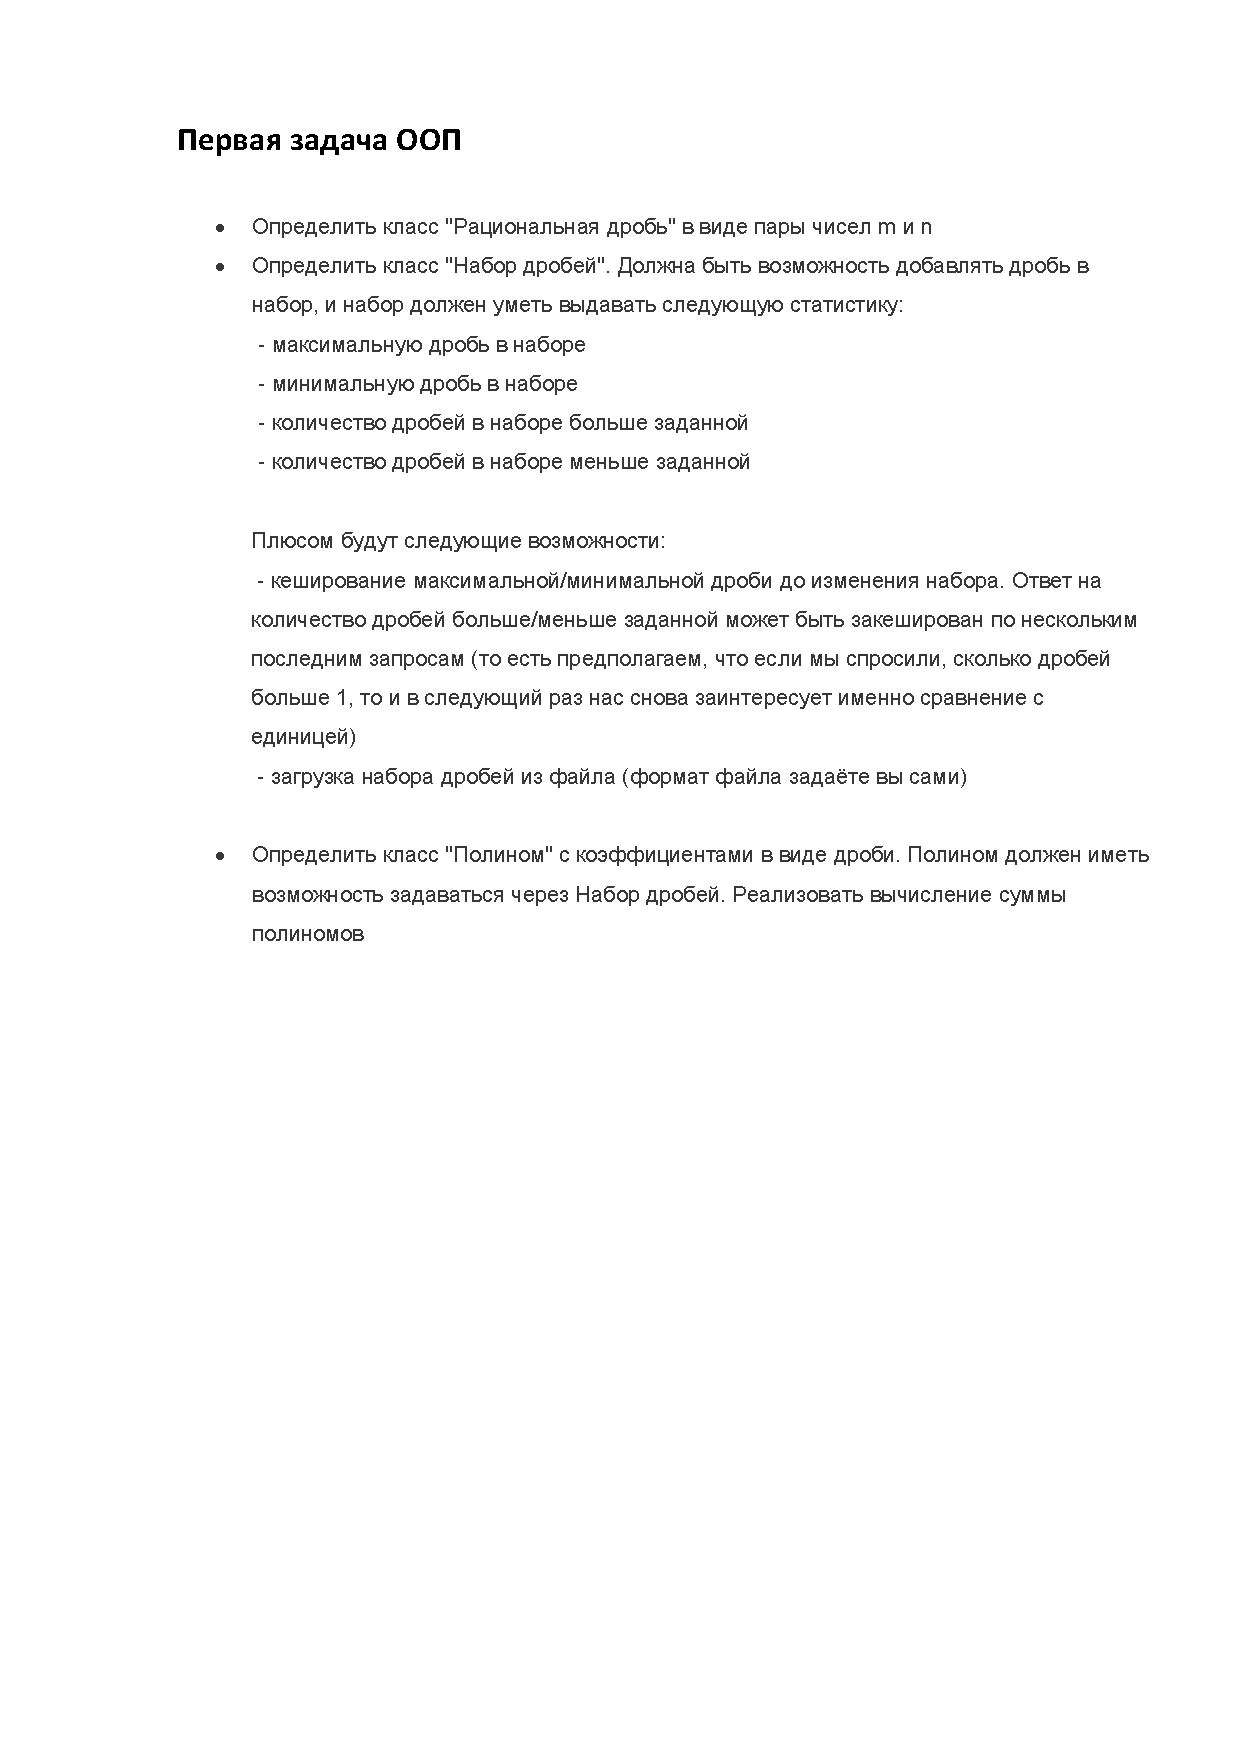
\includepdf[pages=-]{input.pdf} 
\section{Program.cs}
\lstinputlisting{../Program.cs} 
\newpage
\section{Polynomial.cs}
\lstinputlisting{../Polynomial.cs} 
\newpage
\section{RaionalFraction.cs}
\lstinputlisting{../RaionalFraction.cs} 
\newpage
\section{SetFractions.cs}
\lstinputlisting{../SetFractions.cs} 

\newpage\end{document}
